\chapter{Cuerpo del trabajo}

En este apartado desarrollaré en detalle todo el proceso de la creación del videojuego, se dividirá en las siguientes partes:

\begin{enumerate}
	\item Un apartado donde hablaré de las herramientas disponibles, así como la elección que se ha hecho entre todas ellas y su justificación.
	\item Una sección donde estará redactado el \ac{GDD}, en el que hablaré del juego y todas las características del mismo que van a ser implementadas.
	\item Por último, un apartado donde hablaré del desarrollo y la implementación del videojuego, acompañado de explicaciones e imágenes para que se puede apreciar que se ha hecho y de que manera.

\end{enumerate}

\section{Análisis y elección de herramientas para el desarrollo}

En el desarrollo de este proyecto se van a necesitar varios programas con distintas funcionalidades, quiero destacar entre ellos un programa que sea el \textbf{motor del videojuego}, otro que sea para \textbf{modelar} y por último uno que sirva para \textbf{texturizar}.

\subsection{Motor de videojuegos}

Los \textbf{motores de videojuegos} o \textbf{\textit{Game engines}} son \textit{software} diseñados para la creación y desarrollo de videojuegos, ya sea para juegos móvil, para consolas o para ordenadores. Estos motores suelen proveer todo lo necesario para la creación de videojuegos, como motores de físicas para el calculo colisiones o \textit{renderers} para la visualización de los gráficos 2D o 3D.
\\



Hay un número enorme de motores de videojuegos (como podemos apreciar en la imagen a continuación), por lo que para la elección se han tenido en cuenta sólo los dos motores de videojuego comerciales más utilizados en la industria, que son \textbf{\textit{Unity}} y \textbf{\textit{Unreal Engine 4}}.
	
	\begin{figure}[H]
		
				\vspace{-10pt}
		\begin{center}
			
			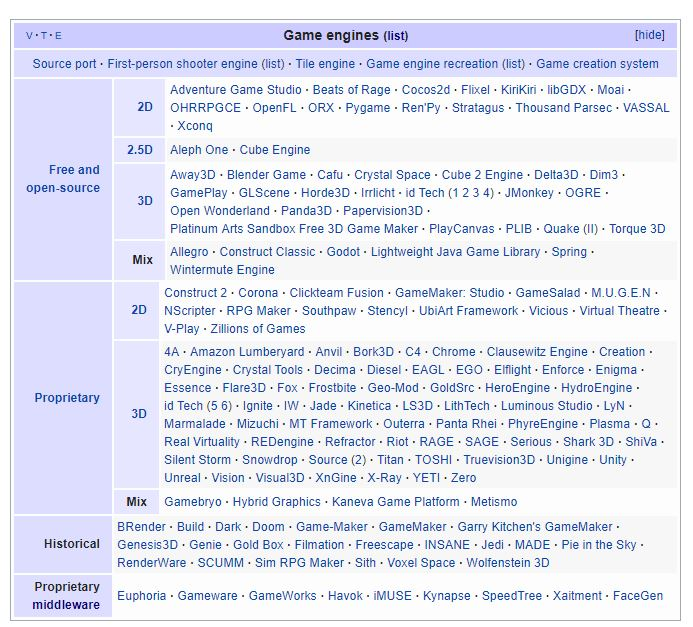
\includegraphics[width=0.85\textwidth]{imagenes/listaMotores.jpg}
			\caption{Lista de grandes motores de juego y sus licencias.}
		\end{center}
		\vspace{-40pt}
	\end{figure}
	
\subsubsection{\textit{Unity}}

\textbf{\textit{Unity}} es un motor de videojuegos creado por \textit{\textbf{Unity Technologies}} y disponible para Windows, macOS y Linux. Unity tiene dos versiones: \textit{Unity Professional} y \textit{Unity Personal}.
\\

\begin{wrapfigure}{i}{0.5\textwidth}
					\vspace{-10pt}
	\begin{center}
						\vspace{-10pt}
		\includegraphics[width=0.55\textwidth]{imagenes/unityLogo.png}
		\caption{Logo de \textit{Unity}.}
						\vspace{-10pt}
	\end{center}
					\vspace{-30pt}
\end{wrapfigure}


\textit{Unity} puede usarse con gran variedad de \textit{software}, como \textit{Blender},\textit{ 3ds Max}, \textit{Maya}, \textit{ZBrush}, \textit{Photoshop}, etc. Los cambios que se realicen a los objetos creados con estos programas se actualizan automáticamente en todo el proyecto sin necesidad de volver a importarlos.
\\


Hoy en día \textit{Unity} tiene un peso muy importante en la industria a la hora de desarrollar juegos, muchos grandes proyectos deciden usar este motor para sus videojuegos, como \textit{\textbf{Hearthstone}} o \textit{\textbf{Furi}}, juegos de gran éxito de ventas y crítica.
\\

No obstante, \textit{Unity} tiene más peso en el sector móvil que en el desarrollo de juegos para ordenadores personales, así que ese motivo junto con la falta de experiencia previa con el motor ha hecho que me decante por \textit{Unreal Engine 4} a la hora de desarrollar el \ac{TFG}.




\subsubsection{\textit{Unreal Engine 4}}
	
\textbf{\textit{Unreal Engine}} es un motor de videojuegos creado por la compañía \textbf{\textit{Epic Games}}, desarrolladora de juegos como \textbf{\textit{Gears of war}} o \textbf{\textit{Unreal Tournament}}.
\\


\begin{wrapfigure}{i}{0.6\textwidth}
	\vspace{-30pt}
	\begin{center}
		\vspace{-10pt}
		
\includegraphics[width=0.55\textwidth]{imagenes/unrealLogo.jpg}
		\caption{Logo de \textit{Unreal Engine 4}.}
	\vspace{-10pt}
	\end{center}
	\vspace{-30pt}
\end{wrapfigure}

La versión actual de \textit{Unreal} está programada en C++ y es compatible con OpenGL y con DirectX 11 y 12. Esta disponible para Windows, Linux y macOS. Además, \textit{Unreal Engine} ofrece herramientas para diseñadores y artistas facilitando la visualización de entornos o de construcciones, lo que ha permitido que \textit{Unreal} se use también en empresas de arquitectura o incluso animación.
\\

\textit{Unreal Engine} es muy utilizado en la industria, hasta el punto que grandes éxitos como los \textit{\textbf{Bioshock}}, \textit{\textbf{Outlast}} e incluso el reciente \textit{\textbf{PlayerUnknown's Battlegrounds}} usen este motor.
\\

\textbf{He decidido usar este motor} precisamente por el gran uso que se tiene de él por parte de las empresas, además de que ya tenía experiencia previa con él, lo que me permitirá acabar con un producto final más redondo. También ha sido determinante en mi elección el sobresaliente acabado final que otorga \textit{Unreal} a los juegos, muy por encima de la mayoría de motores de videojuegos.
\\

\subsection{Programa de modelado}

En gráficos 3D por ordenador, el \textbf{modelado 3D} es el proceso de desarrollo de una una representación matemática de cualquier objeto tridimensional a través de un \textbf{\textit{software} especializado}. Estos modelos pueden ser usado en muchas áreas, como el cine o en la impresión 3D, sin embargo, la utilidad que estamos buscando nosotros es de desarrollo modelos para \textbf{videojuegos}.
\\

\begin{figure}[H]
	
	\vspace{-10pt}
	\begin{center}
		
		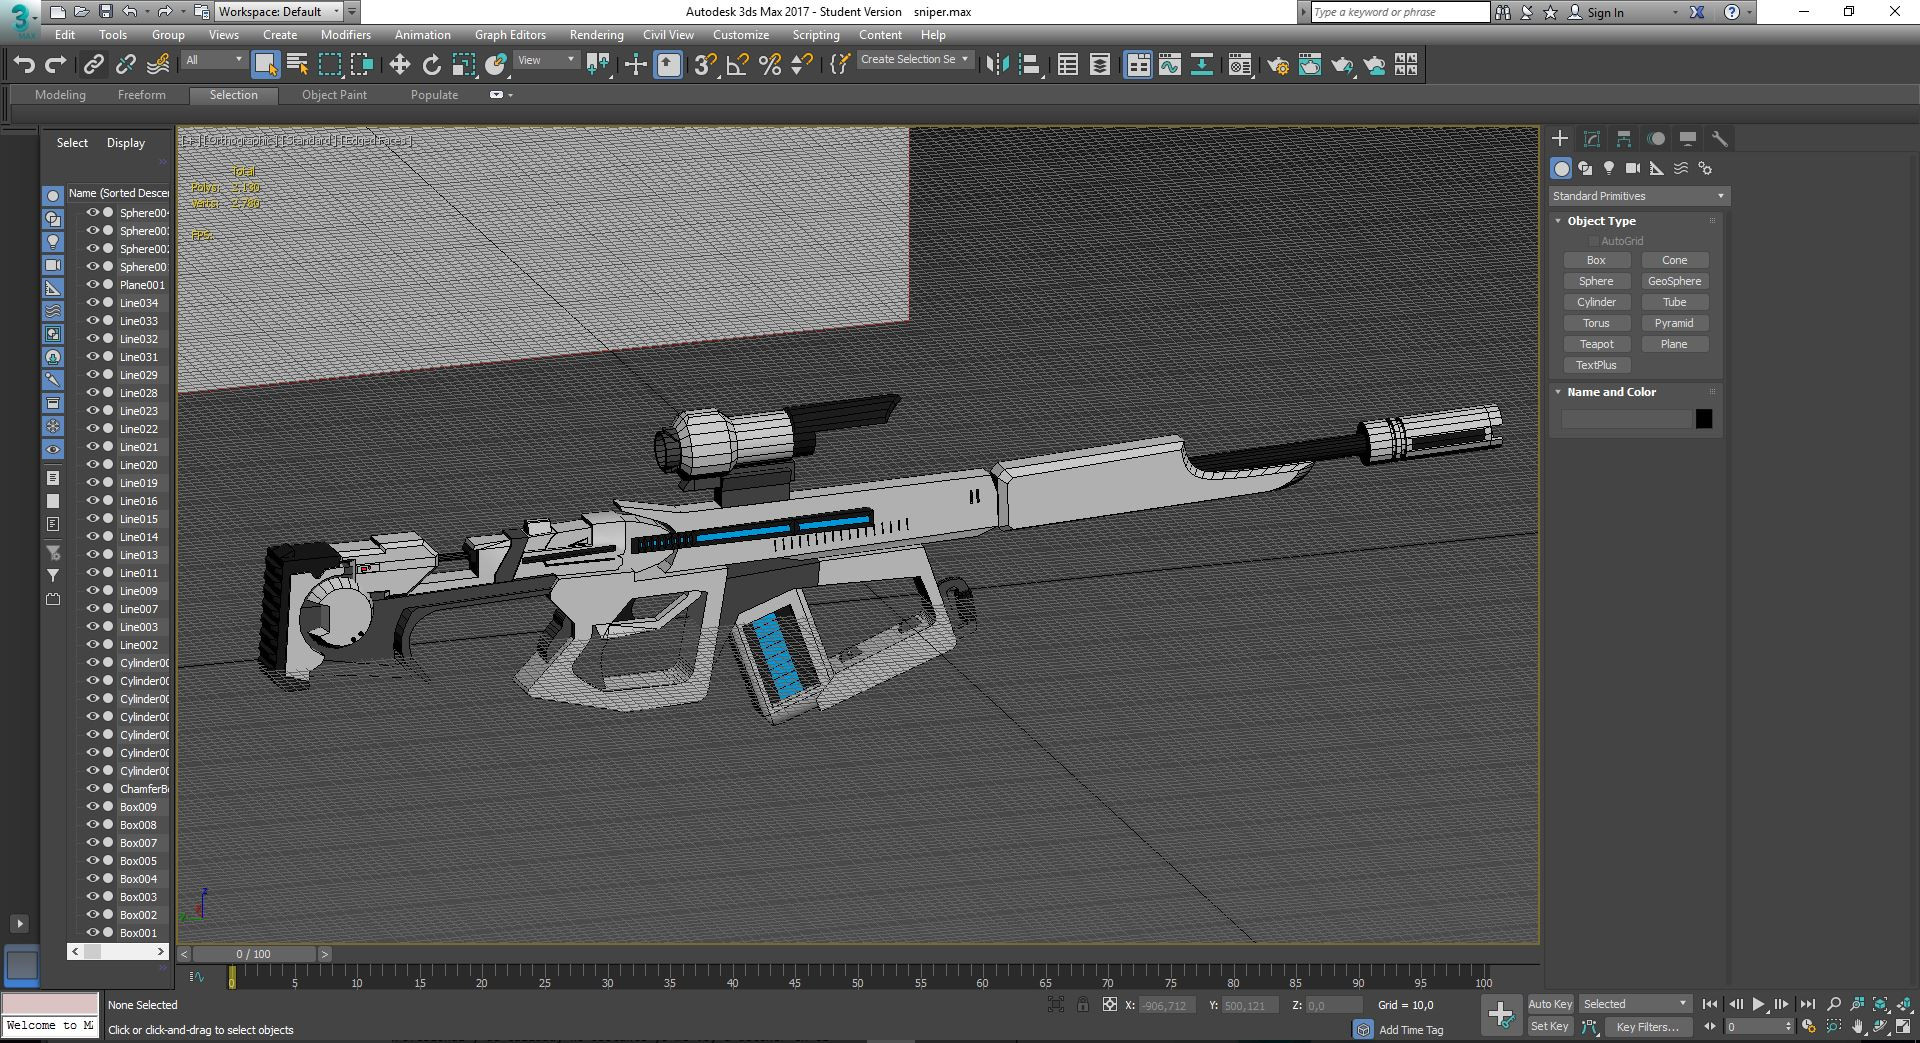
\includegraphics[width=0.9\textwidth]{imagenes/ejemploModelo.jpg}
		\caption{Imagen de un modelo desarrollado por \textit{3ds Max}.}
	\end{center}
	\vspace{-40pt}
\end{figure}

Hay muchos programas de modelado que permiten realizar recursos con un acabado profesional y de calidad, no obstante yo me voy a detener en el \textbf{\textit{Blender}}, el \textbf{\textit{3ds Max}} y el \textbf{Maya\textit{}}, ya que son tres \textit{software} de modelado muy utilizados en la industria.
\\

\subsubsection{\textit{Blender}}

\textit{\textbf{Blender}} es un programa multiplataforma, dedicado especialmente al modelado, iluminación, renderizado, animación y creación de \textbf{gráficos tridimensionales}. \textit{Blender} es un programa de \textbf{software libre}, compatible con \textit{Windows}, \textit{macOS}, \textit{GNU/Linux}, \textit{Solaris}, \textit{FreeBSD} e \textit{IRIX}.
\\

\begin{wrapfigure}{i}{0.6\textwidth}
	\vspace{-30pt}
	\begin{center}
		\vspace{-10pt}
		
\includegraphics[width=0.55\textwidth]{imagenes/blenderLogo.png}
		\caption{Logo de \textit{Blender}.}
		\vspace{-10pt}
	\end{center}
	\vspace{-30pt}
\end{wrapfigure}

\textit{Blender} es un programa muy usado en la industria por pequeñas empresas, ya que el hecho de que sea gratuito lo hace muy apetecible para proyectos de poco presupuesto. También es usado en la industria del cine en películas como \textbf{Spider-man 2} o \textbf{Capitán América: El Soldado de Invierno}.
\\

No obstante, en mi opinión y experiencia previa es un programa mucho más limitado e incómodo que otros \textit{software} de modelado como Maya o 3ds Max, y como puedo utilizar estos dos programas gracias a mi licencia de estudiante no usaré Blender para la realización de este proyecto.
\\

\subsubsection{\textit{Autodesk Maya}}
	
\textbf{\textit{Autodesk Maya}} es un programa dedicado al desarrollo de gráficos 3D por ordenador, efectos especiales y animación creado por \textit{Autodesk}. Esta disponible para \textit{Windows}, \textit{GNU/Linux} y \textit{macOS}.
\\

\begin{wrapfigure}{l}{0.6\textwidth}
	\vspace{-30pt}
	\begin{center}
		\vspace{-30pt}
		
\includegraphics[width=0.35\textwidth]{imagenes/mayaLogo.jpg}
		\caption{Logo de \textit{Autodesk Maya}.}
		\vspace{-20pt}
	\end{center}
	\vspace{-30pt}
\end{wrapfigure}

Este \textit{software} ha tenido un impacto impresionante en la industria del cine, siendo usado en grandes producciones como \textit{\textbf{Jurassic Park}} o \textbf{\textit{Terminator 2}}. Hoy en día prácticamente todas las grandes producciones de Hollywood usan \textit{Maya} para sus efectos especiales.
\\

Sin embargo, aunque este programa tiene una importancia vital en el mundo del cine, \textit{3ds Max} es mucho más usado en el mundo del desarrollo de videojuegos, además, mi experiencia con Maya es mucho más reducida que con 3ds Max.
\\	
	
\subsubsection{\textit{Autodesk 3ds Max}}
	
	
	\begin{wrapfigure}{r}{0.6\textwidth}
		\vspace{-30pt}
		\begin{center}
			\vspace{-30pt}
			
\includegraphics[width=0.35\textwidth]{imagenes/3dsMaxLogo.jpg}
			\caption{Logo de \textit{Autodesk 3ds Max}.}
			\vspace{-20pt}
		\end{center}
		\vspace{-30pt}
	\end{wrapfigure}

\textbf{\textit{Autodesk 3ds Max}} es un programa de creación de gráficos y animación 3D también desarrollado por \textit{Autodesk}. Es uno de los programas de modelado y animación 3D usados en la creación de videojuegos.
\\
	
Aunque es un programa principalmente usado en la industria del videojuego, también ha sido muy usado para anuncios, programas de televisión o películas, destacando \textbf{\textit{Avatar}} o \textbf{\textit{Spider-man 3}}.
\\

\textbf{Esta es la opción que he elegido}, ya que, como he dicho anteriormente, es el \textit{software} más utilizado a día de hoy en el desarrollo de videojuegos. Además, también es el programa con el que tengo más experiencia modelando, por lo que puedo conseguir modelos de calidad en menos tiempo del que necesitaría usando otros programas.
\\
	
	
	
	
	\subsection{Programa de texturizado}
	
\textbf{Texturizar} consiste en crear una \textbf{imagen de mapa de bits} para que cubra la superficie de un objeto virtual, es decir, un modelo. De este modo se le añade detalle al modelo, haciendo que se asemeje más a un objeto real.
\\

	\begin{figure}[H]
		
		\vspace{-10pt}
		\begin{center}
			
			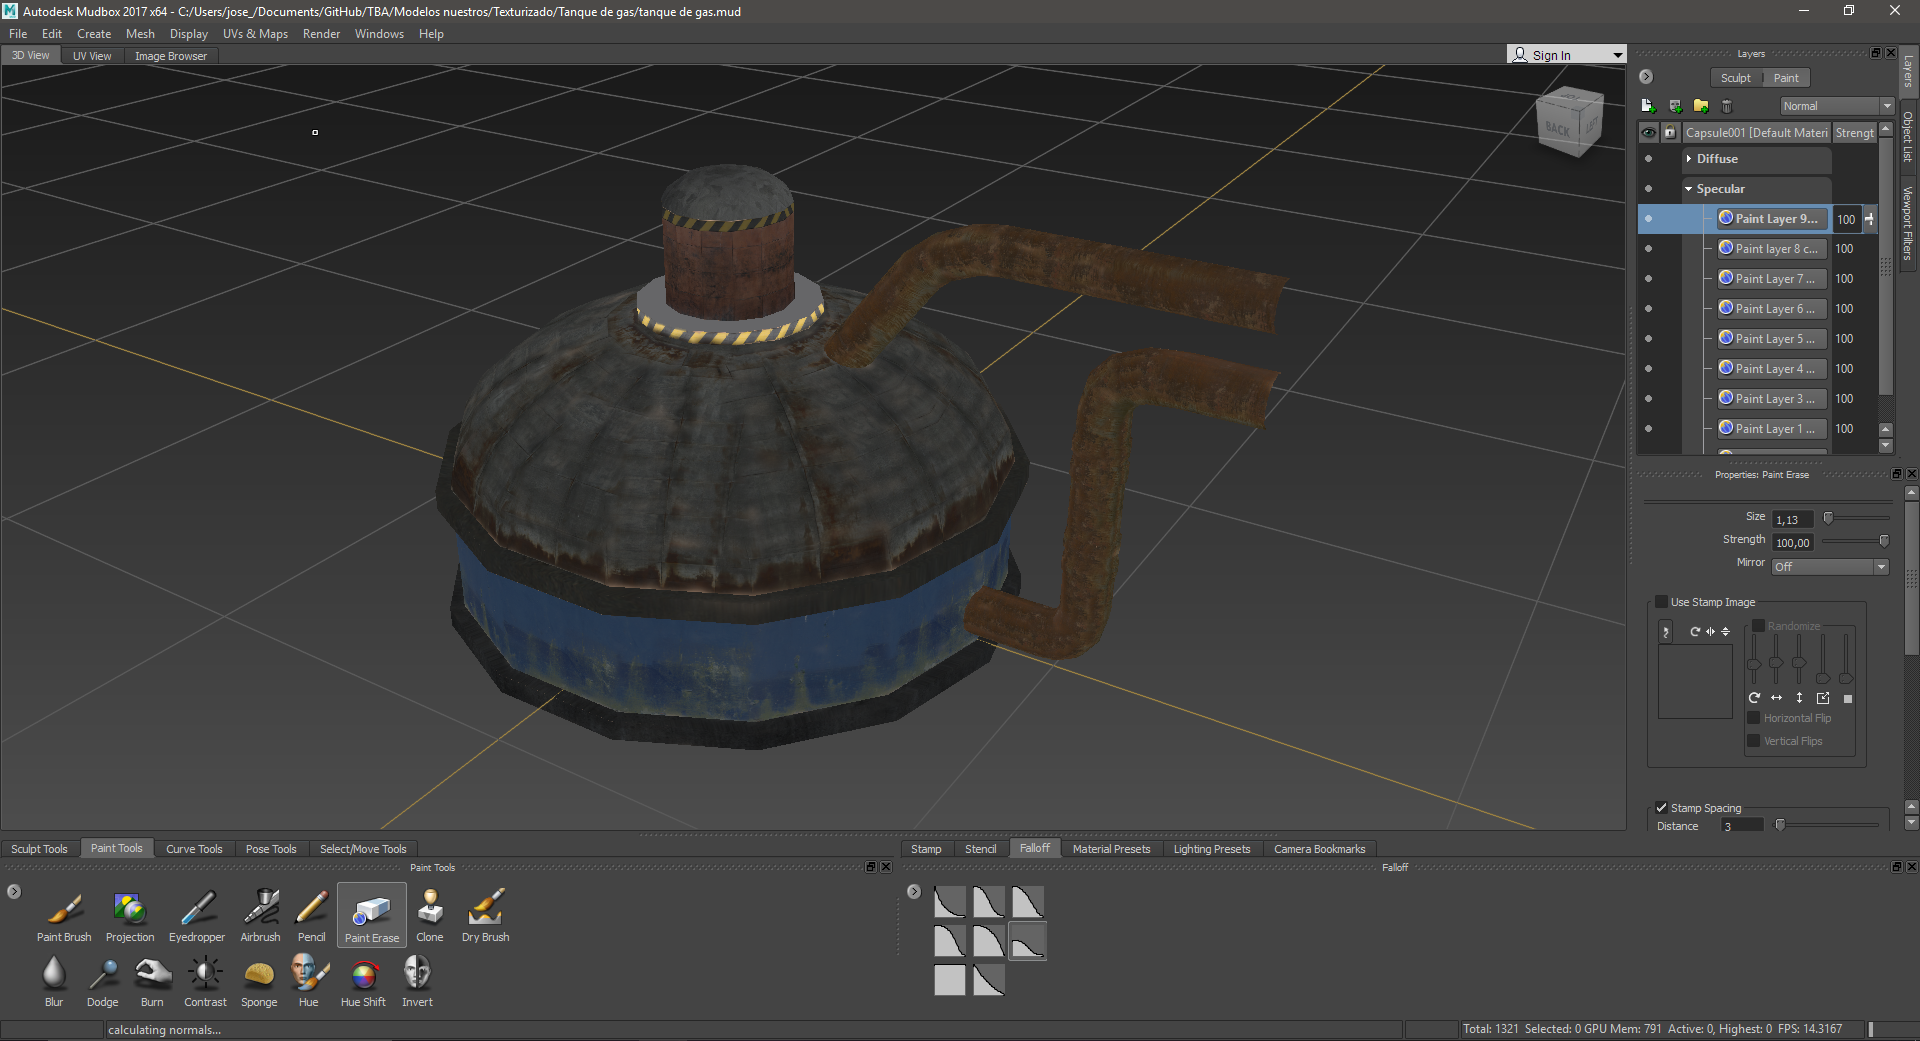
\includegraphics[width=0.9\textwidth]{imagenes/MudboxCapture.png}
			\caption{Imagen de un modelo siendo texturizado en \textit{Mudbox}.}
		\end{center}
		\vspace{-40pt}
	\end{figure}
	
Hay diversos programas que permiten texturizar, incluso algunos que he mencionado anteriormente como 3ds Max tienen herramientas para el texturizado, no obstante existen \textit{software} más especializados y que ofrecen un abanico de posibilidades mayor, como son \textbf{Substance painter} o \textbf{Mudbox}.
\\
	
	\subsubsection{\textit{Substance painter}}
	
	\textit{\textbf{Substance painter}} es un programa de texturizado que está creciendo cada vez más dentro del mercado, que consigue resultados impresionantes de manera sencilla e intuitiva. Está disponible en \textit{Windows}, \textit{macOS} y \textit{Linux}.
	\\
	
	\begin{wrapfigure}{i}{0.6\textwidth}
		\vspace{-30pt}
		\begin{center}
			\vspace{-10pt}
			
\includegraphics[width=0.5\textwidth]{imagenes/substanceLogo.png}
			\caption{Logo de \textit{Substance painter}.}
			\vspace{-10pt}
		\end{center}
		\vspace{-30pt}
	\end{wrapfigure}
	
Una pega del \textit{Substance painter} es que, aunque está creciendo a buen ritmo, su uso en la industria sigue siendo menor. También, al ser un programa no muy utilizado, se pueden encontrar menos recursos y tutoriales para el aprendizaje que los que encuentras para otros programas.
\\
	
Debido a estas razones y a la falta total de experiencia, \textit{Substance painter} ha sido descartado para el uso del producto final, sin embargo, me ha parecido lo suficientemente interesante y destacable como para mencionarlo en esta memoria.
\\


	\subsubsection{\textit{Autodesk Mudbox}}

\textit{\textbf{Autodesk Mudbox}} es un programa de modelado 3D, texturizado y pintura digital desarrollado por \textit{Autodesk}, fue usado por primera vez en la película \textbf{\textit{King Kong} (2005)}. Mudbox funciona perfectamente en sistemas operativos como \textit{Windows}, \textit{Linux} y \textit{macOS}.
\\

\begin{wrapfigure}{r}{0.6\textwidth}
	\vspace{-30pt}
	\begin{center}
		\vspace{-10pt}
		
\includegraphics[width=0.4\textwidth]{imagenes/mudboxLogo.png}
		\caption{Logo de \textit{Autodesk Mudbox}.}
		\vspace{-10pt}
	\end{center}
	\vspace{-30pt}
\end{wrapfigure}

Al ser un programa de \textit{Autodesk}, \textit{Mudbox} tiene mucho más uso en la industria que el que tiene \textit{Substance painter}, siendo mucho más atractivo aprender a usarlo a la hora de incorporarse al mundo laboral el día de mañana.
\\

He decidido \textbf{usar este \textit{software}} precisamente por eso, ya que puede aportarme mucho más en el futuro que \textit{substance painter}, por no hablar que ya tengo cierta base a la hora de usarlo aprendida a lo largo del último año de carrera.
\\


\section{\textit{Game Desing Document} (GDD)}
	
El\textbf{ Documento de Diseño del Juego} (o \textit{Game Design Document}) es el documento en el que se sintetiza todos los componentes y características del juego (concepto, historia, género, niveles...)

Hay muchas maneras y plantillas a la hora de realizar un GDD, no hay una manera fija de esquematizar las diferentes partes del mismo, así que yo voy a seguir el siguiente orden:

\begin{enumerate}
	\item Título y concepto del juego.
		\subitem Título.
		\subitem Historia y argumento.
		\subitem Conjunto de características.
	\item Desarrolladores y género.
		\subitem Desarrolladores.
		\subitem Género.
	\item Plataforma.
	\item Jugabilidad y contenido.
		\subitem Jugabilidad.
		\subitem Objetivos del juego.
		\subitem Progresión.
		\subitem Acciones del personaje.
		\subitem Mecánicas.
		\subitem Controles.
		\subitem Nivel del juego.
		\subitem Apariencia del juego.
	\item Tecnología.
	\item Público.
\end{enumerate}

\subsection{Título y concepto del juego}

\subsubsection{Título}

Lorem Ipsum es simplemente el texto de relleno de las imprentas y archivos de texto. Lorem Ipsum ha sido el texto de relleno estándar de las industrias desde el año 1500, cuando un impresor (N. del T. persona que se dedica a la imprenta) desconocido usó una galería de textos y los mezcló de tal manera que logró hacer un libro de textos especimen. No sólo sobrevivió 500 años, sino que tambien ingresó como texto de relleno en documentos electrónicos, quedando esencialmente igual al original. Fue popularizado en los 60s con la creación de las hojas "Letraset", las cuales contenian pasajes de Lorem Ipsum, y más recientemente con software de autoedición, como por ejemplo Aldus PageMaker, el cual incluye versiones de Lorem Ipsum.
\\

\subsubsection{Historia y argumento}

Nos despertamos desorientados en una pequeña celda oscura y mugrienta, no sabemos que hacemos ahí, solo que\textbf{ estamos en peligro}.
\\

Según escapes de la celda y avances en el juego verás que estas atrapado en una casa de la cual no puedes salir, dónde pasan cosas extrañas, \textbf{tienes que escapar cuanto antes de ahí}.

\subsubsection{Conjunto de características}

Las principales características del juego son:

\begin{itemize}
	\item Ambientación oscura y realista.
	\item Compatible con \textbf{Oculus Rift}.
	\item Desarrollado con \textbf{Unreal Engine 4}
	\item Diseño de niveles centrado en descubrir nuevas localizaciones y salas.
	\item Nivel lleno de detalles.
	\item Mecánicas sencillas y fáciles de aprender.
	\item Diseño sonoro destacable e inmersivo.
\end{itemize}


\subsection{Desarrolladores y género}

\subsubsection{Desarrolladores}

\textbf{\nombreJuego} es un videojuego desarrollado individualmente por José Luis Muñoz Periñán como Trabajo de Fin de Grado de la carrera ingeniería multimedia. Tiene fines puramente académicos y no está previsto ningún uso comercial del producto final.

\subsubsection{Género}

\nombreJuego pertenece al género de los juegos de miedo o \textbf{\textit{survival horror}}.
\\

El juego es una aventura en primera persona inspirada en muchos juegos de miedo de gran éxito en los últimos años, como \textit{Outlast}, \textit{P.T.} o el más reciente \textit{Resident Evil VII}. Se mirarán también como funcionan algunos videojuegos de miedo desarrollados o adaptados para realidad virtual, ya que \nombreJuego estará totalmente adaptado para realidad virtual.
\\

La atmósfera, diseño de mecánicas, apartado artístico y demás características del videojuego estarán enfocadas de acuerdo al género del juego.
\\

\subsection{Plataforma}

\nombreJuego es un videojuego creado en \textit{Unreal Engine 4} desarrollado para ordenadores personales y compatible con las gafas\textit{Oculus Rift}. Cabe destacar que el juego será perfectamente jugable dispongas o no del dispositivo de realidad virtual.
\\

\subsection{Jugabilidad y contenido}

\subsubsection{Jugabilidad}

La jugabilidad será la semejante a la que estamos acostumbrados en los juegos de terror moderno. El protagonista será alguien indefenso y sin recursos ante una situación tenebrosa y que le supera. Unicamente podrá investigar los alrededores e interactuar con el entorno para intentar salir de esa situación. 
\\

Será un juego con mecánicas limitadas para aumentar la sensación de indefensión del jugador e incrementar el terror que el juego provoca.
\\

\subsubsection{Objetivos del juego}

Como he dicho anteriormente, el protagonista está encerrado en una celda de una casa tenebrosa y su objetivo es intentar salir de ahí por todos los medios posibles. A lo largo del juego habrá varios obstáculos que intentarán impedir que alcance su objetivo, como puzzles o momentos de tensión que tendrá que superar usando su ingenio y los objetos que encuentre en el escenario.
\\

\subsubsection{Progresión}

Lorem Ipsum es simplemente el texto de relleno de las imprentas y archivos de texto. Lorem Ipsum ha sido el texto de relleno estándar de las industrias desde el año 1500, cuando un impresor (N. del T. persona que se dedica a la imprenta) desconocido usó una galería de textos y los mezcló de tal manera que logró hacer un libro de textos espécimen. No sólo sobrevivió 500 años, sino que también ingresó como texto de relleno en documentos electrónicos, quedando esencialmente igual al original.
\\

\subsubsection{Acciones del personaje}

El jugador podrá moverse libremente por todo el escenario sin límites, esto es importante ya que el entorno juega un papel importantísimo en el juego, ya que el jugador también podrá coger y usar los objetos de interés que encuentre en el nivel. Por último el jugador también podrá inspeccionar detalladamente algunos objetos específicos que tengan pistas más escondidas moviéndolos y girándolos enfrente suya.
\\

\subsubsection{Mecánicas}

\subsubsection{Controles}

\subsubsection{Nivel del juego}

\subsubsection{Flujo del juego}

\subsubsection{Apariencia del juego}

\subsection{Tecnología}

\subsection{Público}
